\documentclass[conference]{IEEEtran}
\IEEEoverridecommandlockouts
\usepackage{cite}
\usepackage{amsmath,amssymb,amsfonts}
\usepackage{algorithmic}
\usepackage{graphicx}
\usepackage{textcomp}
\usepackage{xcolor}
\usepackage{tikz}
\usetikzlibrary{arrows.meta, positioning, shapes.geometric}
\sloppy
\usepackage{threeparttable}

\usepackage{times}
\setlength{\textfloatsep}{6pt plus 1pt minus 1pt}
\setlength{\floatsep}{4pt plus 1pt minus 1pt}
\setlength{\intextsep}{6pt plus 1pt minus 1pt}
\setlength{\abovecaptionskip}{3pt}
\setlength{\belowcaptionskip}{2pt}

\def\BibTeX{{\rm B\kern-.05em{\sc i\kern-.025em b}\kern-.08em
T\kern-.1667em\lower.7ex\hbox{E}\kern-.125emX}}
\begin{document}

\title{BD-HAR: A Bangladeshi Smartphone Sensor Dataset for Human Activity Recognition and Cross-Dataset Evaluation with UCI-HAR}

% Check the author block before submission (double-blind: remove for initial submission)
%\author{
%\IEEEauthorblockN{Md Shahidul Islam$^1$, S M Tamzid Islam$^2$, Rabbi Mushad$^3$, Md Tauhidur Rahman$^4$, Nusrat Sharmin$^5$}
%\IEEEauthorblockA{
%$^{1,2,3,4,5}$\textit{Department of Computer Science and Engineering}\\
%\textit{Military Institute of Science and Technology (MIST)}, Dhaka, Bangladesh\\
%Email: rony6552@gmail.com, shagor57@gmail.com, mushad9822@gmail.com, tauhid10451@gmail.com, nusrat@cse.mist.ac.bd
%}
%}


\maketitle

\begin{abstract}
Human Activity Recognition (HAR) using smartphone sensors is widely applied in healthcare monitoring, fall detection, and fitness tracking. However, most existing HAR benchmarks, such as UCI-HAR, WISDM, and PAMAP2, are collected from Western or East Asian populations and do not represent the phone-handling habits or body composition of Bangladeshi users. The only existing Bangladeshi dataset, KU-HAR, uses an incompatible activity scheme and releases no participant demographic metadata, preventing controlled cross-dataset evaluation. To address this gap, we introduce BD-HAR, an real-world Bangladeshi smartphone sensor dataset comprising 5,507 labelled activity windows from 21 volunteers performing six activities under natural phone placement (Hand, Trouser Pocket), along with age, height, weight, and BMI collected in-person. This dataset enables cross-population benchmarking of HAR models between Bangladeshi and international populations. BD-HAR was evaluated using ML models (SVM, Random Forest, KNN) and DL models (MLP, 1D CNN) under within-dataset and cross-dataset protocols against UCI-HAR, with deep models reaching up to 90.2\% within-dataset accuracy but only 14-33\% under cross-dataset transfer, exposing substantial domain shift between populations. This paper presents applications and future directions using our proposed dataset to advance population-aware HAR research for Bangladesh.
\end{abstract}

\begin{IEEEkeywords}
human activity recognition dataset, smartphone sensors, Bangladeshi dataset, domain shift, machine learning, deep learning
\end{IEEEkeywords}

\section{Introduction}
\label{sec:intro}

Smartphones equipped with accelerometers and gyroscopes can be
segmented into windows to build Human Activity Recognition (HAR)
datasets, a practical and widely studied problem
\cite{anguita_public_2013} used in healthcare monitoring, fall
detection and fitness tracking~\cite{martins_elderhar_2026,
miah_sensor_based_2024, alanazi_human_2024}. The same activity performed by different individuals produces different sensor signatures, and this variability is amplified when models trained on one population are deployed on another.

Most widely-used smartphone-based HAR benchmarks, including
UCI-HAR~\cite{anguita_public_2013}, WISDM~\cite{kwapisz_activity_2011}
and PAMAP2~\cite{reiss_introducing_2012}, were collected from European,
North American or East Asian volunteers, as summarized in
Table~\ref{tab:dataset_compare}. A Bangladeshi dataset, KU-HAR
\cite{sikder_kuhar_2021}, exists but uses 18 heterogeneous activities
that do not map onto UCI-HAR's 6-class label scheme and released no
participant-level placement, age, or anthropometric metadata, making
it unsuitable for controlled, label-aligned cross-dataset transfer or
metadata-driven subgroup analysis. This matters because cross-dataset
studies consistently show HAR models degrade when transferred across
populations~\cite{hong_crosshar_2024, napoli_benchmark_2024}, and body composition remains an untested contributor to this degradation. To address this critical
gap, we introduce BD-HAR, a novel dataset comprising 5{,}507 labelled
sensor windows from 21 Bangladeshi volunteers, collected under
naturalistic phone placement with accompanying age, height, weight,
BMI and placement metadata.

\begin{table*}[t]
\centering
\footnotesize
\setlength{\tabcolsep}{5pt}
\begin{threeparttable}
\caption{Comparison of BD-HAR with existing HAR benchmarks.}
\label{tab:dataset_compare}
\begin{tabular}{lccccc}
\hline
Metric & UCI-HAR & WISDM & PAMAP2 & KU-HAR & BD-HAR \\
\hline
Region & Italy & USA & Germany & Bangladesh & Bangladesh \\
Subjects & 30 & 29 & 9 & 90 & 21 \\
Activities & 6 & 6 & 18 & 18 & 6 \\
Sampling rate & 50 Hz & 20 Hz & 100 Hz & 100 Hz & 50 Hz \\
Sensor placement & Waist & Pocket & Wrist/chest/ankle & Self-selected & Hand/pocket \\
Age metadata & No & No & No & No & Yes \\
Height/weight/BMI metadata & No & No & Partial & No & Yes \\
Public availability & Public & Public & Public & Public & Public* \\
\hline
\end{tabular}
\begin{tablenotes}
\footnotesize
\item[$^{*}$] Released upon publication; see Data Availability Statement.
\end{tablenotes}
\end{threeparttable}
\end{table*}

The main contributions of this research are outlined as follows:
\begin{itemize}
\item Development of BD-HAR, the first Bangladeshi HAR dataset
explicitly aligned to UCI-HAR's 6-activity label scheme, collected
from 21 volunteers with rigorously annotated participant-level age,
height, weight, BMI and phone-placement metadata (5{,}507 usable labelled
windows) enabling demographic and anthropometric subgroup analysis
and direct cross-dataset transfer evaluation that neither UCI-HAR,
WISDM, PAMAP2 nor the existing 18-class KU-HAR benchmark can support.


\item A fully documented, auditable collection protocol, including
an in-app automated sensor-quality check, a two-session
warmup-then-final recording design and direct device-to-cloud upload that supports reproducibility of the collection process itself.

\item As an application of the proposed dataset, a shared,
identically-applied 72-feature extraction pipeline across five models
(SVM, Random Forest, KNN, MLP, 1D CNN), evaluated under both random
(70/30) and subject-independent (LOSO) cross-dataset protocols against
UCI-HAR including a LOSO-based gap decomposition, a bidirectional CORAL baseline, and subgroup and confusion-matrix analyses.
\end{itemize}

\section{Related Work}
\label{sec:background}

This section reviews the benchmark datasets and model architectures
that established smartphone-based HAR as a deep-learning-dominated
field (Section~\ref{subsec:datasets}), before examining why models
trained on these benchmarks fail to generalize across datasets and
populations (Section~\ref{subsec:crossdataset}).

\subsection{Benchmark Datasets and Model Architectures}
\label{subsec:datasets}
Anguita et al.~\cite{anguita_public_2013} established the UCI-HAR
benchmark using 30 Italian volunteers, extracting a 561-feature vector
from waist-mounted sensors and reaching 96\% accuracy with a multiclass
SVM. Kwapisz et al.~\cite{kwapisz_activity_2011} showed a pocket-worn
phone with an MLP reaches 91.7\% on WISDM, though static activities
remained harder. Alanazi et al.~\cite{alanazi_human_2024} confirmed
this pattern on KU-HAR. Deep architectures later improved on these
baselines: Zeng et al.~\cite{zeng_convolutional_2014} showed 1D CNNs with
partial weight sharing outperform hand-crafted features, and Zebin et
al.~\cite{zebin_human_2018} found Batch-Normalized LSTMs cut training
time four-fold without accuracy loss. Most relevant here, Hossain et
al.~\cite{hossain_enhanced_2024} demonstrated a compact deep MLP
reaching 96.81\% on UCI-HAR, outperforming 1D CNN and LSTM baselines but
explicitly noted that generalization beyond UCI-HAR and MotionSense
remains untested. Miah et al.~\cite{miah_sensor_based_2024} achieved 99.9\% with a 4-stream TCN, though at high parameter cost. None of these
benchmarks release participant height, weight or BMI, so the influence
of body composition on HAR accuracy remains largely unexamined in the
literature.

The only existing Bangladeshi smartphone HAR dataset is
KU-HAR~\cite{sikder_kuhar_2021} which collected 90 participants
performing 18 heterogeneous activities (including talking, jumping,
push-ups and table tennis) at 100~Hz, reaching close to 90\% accuracy
with Random Forest on its own held-out data. However, KU-HAR's
18-class label scheme does not align with UCI-HAR's 6 activities,
preventing direct label-matched cross-dataset transfer, and its public
release does not include per-participant placement, age, or
anthropometric metadata. BD-HAR is designed specifically to close this
gap: it mirrors UCI-HAR's 6-activity scheme exactly and logs age,
height, weight, BMI and placement for every participant, enabling the
controlled transfer and subgroup analysis in
Section~\ref{sec:modelapp} that KU-HAR cannot support.

\subsection{Cross-Dataset Generalization}
\label{subsec:crossdataset}
Domain shift, the mismatch between training and test data
distributions, degrades HAR models substantially when transferred
across datasets. Prior work narrows this gap via hierarchical self-supervised pretraining (+10.83\%)\cite{hong_crosshar_2024}, standardized-format benchmarking \cite{napoli_benchmark_2024} and Maximum Mean Discrepancy alignment (+45\% F1) \cite{kasim_cross_domain_2023}, though absolute cross-dataset scores remain low in all three. Sun et al.
\cite{sun_return_2016, sun_correlation_2017} proposed CORrelation
ALignment (CORAL), an unsupervised domain adaptation method that
aligns the second-order statistics (covariances) of source and target
feature distributions without requiring target labels, later extended
to deep networks as a differentiable alignment loss. Unlike
hierarchical pretraining or mix-based augmentation approaches
\cite{hong_crosshar_2024, napoli_domain_2025}, this study adopts CORAL
\cite{sun_return_2016, sun_correlation_2017} as a lightweight
domain-adaptation baseline to demonstrate BD-HAR's value as a
cross-population evaluation benchmark (Section~\ref{sec:modelapp}).
Recent work also shows that random k-fold or fixed-ratio splits can
substantially overestimate HAR performance compared to
subject-independent protocols such as Leave-One-Subject-Out (LOSO),
due to violations of the independent-and-identically-distributed
assumption between temporally adjacent, subject-correlated windows
\cite{tello_too_2023, pang_stacked_2022}; this study therefore reports
LOSO ceilings alongside 70/30 results when validating BD-HAR. Prior
domain adaptation and fairness-aware methods reveal unequal error
rates across demographic subgroups - one study reports a 0.4968
gender-based Equalized Odds gap for running \cite{roy_fairness_2023}
and another finds elderly users misclassified more often during
transitional activities \cite{martins_elderhar_2026} - but both are
drawn only from European populations and neither examines body
composition. No existing study evaluates HAR performance, domain
adaptation, or anthropometric fairness on a Bangladeshi population, a
gap this paper addresses through BD-HAR (Section~\ref{sec:dataset}).

\section{Development of the BD-HAR Dataset}
\label{sec:dataset}

This section provides an extensive overview of the proposed BD-HAR
dataset. Subsection~\ref{subsec:datacollection} describes the data
collection and consent process, Subsection~\ref{subsec:annotation}
explains the annotation and validation procedure, and
Subsection~\ref{subsec:description} describes the resulting dataset
and its metadata, including its anthropometric composition.

\subsection{Data Collection}
\label{subsec:datacollection}
BD-HAR was collected from an initial pool of 25 Bangladeshi adult
volunteers recruited through the authors' professional network, using
a custom Android application that logged tri-axial accelerometer and
gyroscope readings at 50~Hz. Fig.~\ref{fig:collection_flow}
summarizes the end-to-end collection and validation pipeline. Each
volunteer first received a verbal explanation of the study's purpose
and the sensor data being collected, then installed the application
and entered demographic credentials (age, height, weight, gender,
name and mobile number); name and mobile number were recorded only
for session bookkeeping and were permanently removed prior to public
release, leaving no personally identifiable information in the
published dataset, while height and weight were retained to compute
per-participant BMI (Section~\ref{subsec:description}). Each
participant then explicitly acknowledged an in-app consent statement,
presented as a mandatory checkbox during the login step, before any
sensor logging could begin.

Before recording, the app ran an automated sensor-quality check;
4 of the 25 initial volunteers were discarded at this stage due to
faulty accelerometer/gyroscope readings, leaving 21 validated
participants (ages 18-37, mean 24.8, std 5.8). Data collection was
conducted by the authors across two in-person sessions in June 2026,
with two authors physically present throughout: an initial warmup
session verified app performance and oriented participants to the
protocol, followed by a final recording session in which all 21
participants completed the six target activities (Walking, Walking
Upstairs, Walking Downstairs, Sitting, Standing, Lying), matching the
UCI-HAR label scheme~\cite{anguita_public_2013}. For each activity,
participants first performed the activity with the phone held in
Hand, then repeated the same activity with the phone in the Trouser
Pocket; a Chest Pocket option also existed in the app but was
intentionally excluded from the protocol, though a small number of
Chest Pocket recordings were later discovered during analysis and
treated as invalid input (Section~\ref{subsec:annotation}). After each
recorded activity, the app automatically uploaded the session directly
to a central Google Sheets repository, logging timestamp,
participant ID, demographic fields, activity label, phone placement,
six-axis raw sensor readings, session ID, device model, session
duration and sampling rate; a small number of upload failures were
identified and corrected manually by the authors after collection.
Raw sensor streams (443{,}663 readings across 283 sessions) were
collected in total, forming the raw basis of the dataset described
below.

Given the minimal-risk, non-biometric nature of this data, formal
institutional ethics board review was not sought; this is noted as a
limitation (Section~\ref{sec:applications}), and future large-scale
extensions of BD-HAR will pursue formal ethics clearance prior to
collection.

\begin{figure*}[t]
\centering
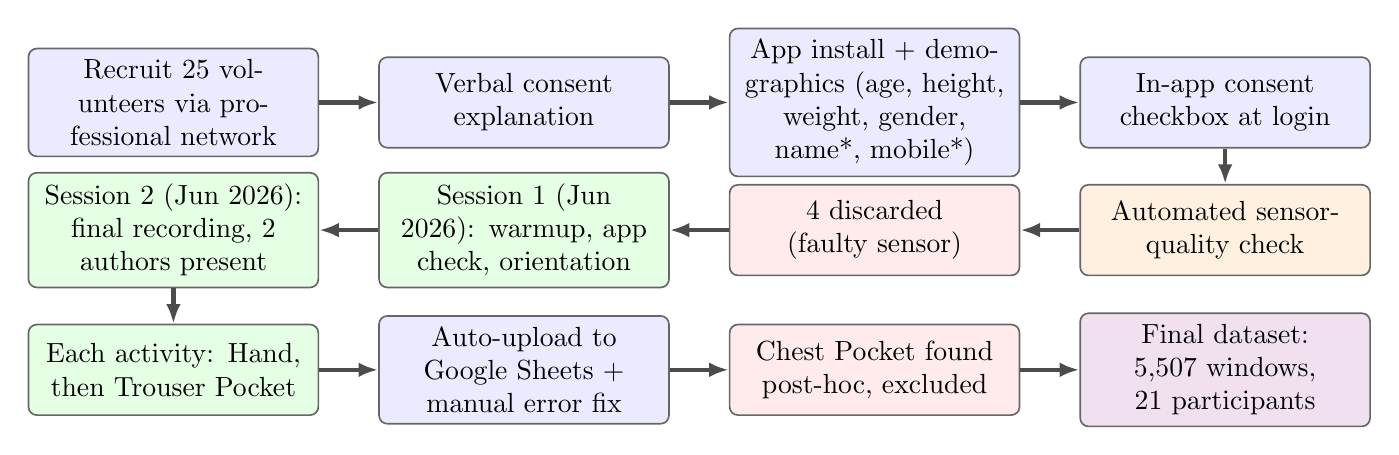
\begin{tikzpicture}[
node distance=0.45cm and 0.75cm,
every node/.style={font=\normalsize},
boxnode/.style={rectangle, rounded corners=3pt, draw=black!60, line width=0.6pt,
minimum width=3.6cm, minimum height=1.15cm,
align=center, text width=3.4cm, inner sep=4pt},
stepnode/.style={boxnode, fill=blue!8},
checknode/.style={boxnode, fill=orange!12},
sessnode/.style={boxnode, fill=green!10},
outnode/.style={boxnode, fill=red!8},
finalnode/.style={boxnode, fill=violet!12},
arrownode/.style={-{Latex[length=2.5mm]}, ultra thick, black!70}
]

\node[stepnode] (recruit) {Recruit 25 volunteers via professional network};
\node[stepnode, right=of recruit] (consent1) {Verbal consent explanation};
\node[stepnode, right=of consent1] (install) {App install + demographics (age, height, weight, gender, name*, mobile*)};
\node[stepnode, right=of install] (consent2) {In-app consent checkbox at login};

\node[checknode, below=of consent2] (sensorcheck) {Automated sensor-quality check};
\node[outnode, left=of sensorcheck] (discard) {4 discarded (faulty sensor)};
\node[sessnode, left=of discard] (sess1) {Session 1 (Jun 2026): warmup, app check, orientation};
\node[sessnode, left=of sess1] (sess2) {Session 2 (Jun 2026): final recording, 2 authors present};

\node[sessnode, below=of sess2] (activity) {Each activity: Hand, then Trouser Pocket};
\node[stepnode, right=of activity] (upload) {Auto-upload to Google Sheets + manual error fix};
\node[outnode, right=of upload] (chest) {Chest Pocket found post-hoc, excluded};
\node[finalnode, right=of chest] (finalbox) {Final dataset: 5{,}507 windows, 21 participants};

\draw[arrownode] (recruit) -- (consent1);
\draw[arrownode] (consent1) -- (install);
\draw[arrownode] (install) -- (consent2);
\draw[arrownode] (consent2) -- (sensorcheck);
\draw[arrownode] (sensorcheck) -- (discard);
\draw[arrownode] (discard) -- (sess1);
\draw[arrownode] (sess1) -- (sess2);
\draw[arrownode] (sess2) -- (activity);
\draw[arrownode] (activity) -- (upload);
\draw[arrownode] (upload) -- (chest);
\draw[arrownode] (chest) -- (finalbox);

\end{tikzpicture}
\caption{BD-HAR data collection and validation pipeline, from
recruitment and consent through the two-session recording protocol to
the final validated dataset. *Name and mobile number removed prior to
public release; height and weight retained for BMI computation.}
\label{fig:collection_flow}
\end{figure*}

\subsection{Dataset Annotation and Validation}
\label{subsec:annotation}
Each recording session was labelled at collection time with the
activity being performed, the participant's self-selected phone
placement, and participant age, ensuring that every raw session in
BD-HAR carries verified ground-truth annotation rather than
post-hoc labelling. Sessions with ambiguous or interrupted activity
performance were flagged during collection and excluded prior to
windowing (Section~\ref{sec:preprocessing}). Chest Pocket sessions
were subsequently identified as unintentionally recorded and were
excluded from all further analysis, leaving Hand and Trouser Pocket as
the two validated placement conditions. Height and weight values
collected at enrollment were validated for physiological plausibility
and converted into BMI (Section~\ref{subsec:description}) using the
standard formula BMI $=$ weight(kg)/height(m)$^2$.

\subsection{Description of the BD-HAR Dataset and Metadata}
\label{subsec:description}
The validated raw sensor streams were segmented into 128-sample
windows (2.56~s at 50~Hz) with 50\% overlap, yielding 6{,}528
labelled windows across all placements. After excluding Chest Pocket
sessions, 5{,}507 usable windows remain (Hand: 2{,}913; Trouser
Pocket: 2{,}594), covering the same six activity classes as UCI-HAR:
Walking, Walking Upstairs, Walking Downstairs, Sitting, Standing and
Lying. In addition to the labelled sensor windows, BD-HAR includes
participant-level metadata: age (18-37 years, mean 24.8, std 5.8),
self-selected phone placement (Hand or Trouser Pocket), and BMI,
computed from height and weight recorded at enrollment. Across the 21
validated participants, BMI ranges from 21.0 to 34.1 (mean 25.8, std
3.4), with 11 participants classified as Normal weight (BMI
18.5-24.9), 7 as Overweight (25-29.9) and 3 as Obese ($\geq$30);
no participants fell in the Underweight range ($<$18.5), which is
noted as a coverage gap in Section~\ref{sec:applications}.
Table~\ref{tab:bmi_dist} summarizes this distribution. This metadata
enables the placement-, age- and BMI-level subgroup analysis reported
in Section~\ref{sec:modelapp}, which is not possible with UCI-HAR,
WISDM, PAMAP2 or KU-HAR, none of which release comparable
participant-level anthropometric metadata. Table~\ref{tab:dataset_compare} situates BD-HAR relative to these benchmarks.

\begin{table}[!t]
\centering
\footnotesize
\caption{BMI distribution across the 21 validated BD-HAR participants.}
\label{tab:bmi_dist}
\begin{tabular}{lccc}
\hline
BMI Category & Range & Count & \% of Sample \\
\hline
Underweight & $<$18.5 & 0 & 0.0\% \\
Normal & 18.5-24.9 & 11 & 52.4\% \\
Overweight & 25.0-29.9 & 7 & 33.3\% \\
Obese & $\geq$30.0 & 3 & 14.3\% \\
\hline
\end{tabular}
\end{table}

\section{Data Preprocessing}
\label{sec:preprocessing}

Before model training, BD-HAR's raw sensor streams were windowed,
filtered, normalized and converted into a feature representation
compatible with UCI-HAR.

\subsection{Windowing and Session Filtering}
Raw sensor streams (443{,}663 readings across 283 sessions) were
segmented into 128-sample windows (2.56~s at 50~Hz) with 50\% overlap
(step size of 64 samples), yielding 6{,}528 labelled windows. Chest
Pocket sessions were discarded intentionally as described in
Section~\ref{subsec:annotation}, leaving 5{,}507 usable windows (Hand:
2{,}913; Trouser Pocket: 2{,}594) for analysis; each participant's BMI
label is propagated to every window derived from their sessions.

\subsection{Feature Extraction and Normalization}
\label{subsec:features}
UCI-HAR's official 561-feature set relies on a dataset-specific
pipeline (gravity/body-acceleration separation, autoregressive
coefficients, angle features) that cannot be consistently reproduced
on new raw sensor data. So a custom 72-feature set was extracted identically from both datasets to guarantee a fair comparison. For each of six sensor
channels (acc\_x, acc\_y, acc\_z, gyro\_x, gyro\_y, gyro\_z), nine
time-domain statistics (mean, standard deviation, maximum, minimum,
median, skewness, kurtosis, RMS, sum of absolute first differences)
and three FFT-based frequency-domain statistics (mean, standard
deviation, maximum) were computed, giving 72 features per window,
following common practice in accelerometer/gyroscope-based
HAR~\cite{issa_har_embedded_2022}. Prior to feature extraction, each
window from both datasets was normalized per channel using per-window
z-score normalization,
\[
x_{\text{norm}} = \frac{x_{\text{raw}} - \mu_{\text{window}}}{\sigma_{\text{window}}},
\]
which removes absolute amplitude and energy differences between
datasets while preserving relative movement shape. The same
72-feature, normalized vector fed all five models in
Section~\ref{subsec:models}, ensuring that observed performance
differences reflect architecture rather than input representation.

\section{Model Implementation (An Application of the BD-HAR Dataset)}
\label{sec:modelapp}

As an application demonstrating BD-HAR's utility, this section
evaluates five widely used algorithms for cross-dataset HAR transfer
between UCI-HAR and BD-HAR, including a subgroup analysis by phone
placement, age and BMI category.

\subsection{Model Architectures and Hyperparameters}
\label{subsec:models}
Five models were trained on the identical 72-feature input: a Support
Vector Machine (SVM, RBF kernel, balanced class weights), a Random
Forest (RF, 200 trees, balanced class weights), a K-Nearest Neighbors
(KNN, $k=5$) classifier, a deep Multi-Layer Perceptron (MLP) adapted
from Hossain et al.~\cite{hossain_enhanced_2024} (hidden layers 64,
36, 12, 36; dropout 0.2; input reduced from 561 to 72), and a
one-dimensional 1D CNN that reshapes each 72-feature vector into a
length-72 single-channel sequence for convolution. The MLP and 1D CNN
were trained with Adam and categorical cross-entropy loss, using
early stopping (patience 10) and other parameters used as standard defaults.

\subsection{Evaluation Protocol}
\label{subsec:evalprotocol}
All five models were evaluated within-dataset on UCI-HAR and BD-HAR
under subject-independent LOSO to establish each dataset's accuracy
ceiling, with MLP and 1D CNN additionally evaluated under a 70/30
stratified split. For cross-dataset evaluation, all five models were
trained on one dataset and evaluated on the other in both directions
(UCI$\rightarrow$BD and BD$\rightarrow$UCI), following prior HAR
transfer protocols~\cite{hong_crosshar_2024,kasim_cross_domain_2023},
with predictions further grouped by phone placement, participant age
group, and BMI category using the metadata in
Section~\ref{subsec:description}. Because age, BMI and placement were
not independently balanced across the 21-participant sample with
some BMI categories (Obese, $n=3$) containing very few individuals
these subgroup effects are reported separately and interpreted as
exploratory and potentially confounded rather than statistically
conclusive.
Finally, CORrelation ALignment (CORAL)~\cite{sun_return_2016} was
applied as a lightweight domain-adaptation baseline, aligning source
and target feature covariances without requiring target labels.

\section{Results}
\label{sec:results}

\subsection{Within-Dataset and Cross-Dataset Performance}
The deep models (MLP, 1D CNN), evaluated within each dataset under a
70/30 split, reached 0.878/0.902 on UCI-HAR but only 0.584/0.582 on
BD-HAR, confirming BD-HAR is intrinsically harder even under matched
train-test conditions and that the adapted MLP reproduces Hossain et
al.'s UCI-HAR performance \cite{hossain_enhanced_2024}; this
difficulty held across both deep and classical models. Bidirectional
cross-dataset accuracy (Source-Only columns,
Table~\ref{tab:baseline_coral_combined}) shows KNN performing best in
both directions, with neither deep model outperforming classical
baselines, pointing to distributional mismatch rather than model
capacity as the main obstacle.

\subsection{Placement, Age and BMI Subgroup Effects}
Phone placement mattered consistently: for UCI$\rightarrow$BD
transfer, Hand outperformed Trouser Pocket across all models (SVM:
0.074 vs.\ 0.211; MLP: 0.099 vs.\ 0.200; 1D CNN: 0.121 vs.\ 0.248). Age
effects were smaller and confounded with placement (KNN: 0.188-0.232
across four age groups). BD-HAR's 21 participants span a BMI range of
21.0-34.1 (Table~\ref{tab:bmi_dist}), but with only 3 participants in
the Obese category, BMI-stratified accuracy is reported here as
descriptive metadata rather than a statistically powered subgroup
comparison; the marked skew toward Normal/Overweight participants
(19 of 21) and complete absence of Underweight participants limits
what can be concluded about body-composition effects from the current
sample, and is flagged as a priority for expansion in
Section~\ref{sec:applications}.

\subsection{Gap Decomposition}
\label{subsec:loso_gap}

Table~\ref{tab:split_compare} reports LOSO and 70/30 accuracy; the
70/30 split consistently overstates performance (e.g., 1D CNN: 0.902 vs.\
0.8287 on UCI-HAR), confirming random splits overestimate accuracy by
leaking subject identity across train/test
\cite{tello_too_2023, pang_stacked_2022}. Table~\ref{tab:gap}
decomposes the LOSO-based UCI$\rightarrow$BD drop: the
dataset-difficulty component (0.377 average) exceeds the domain-shift
component (0.253), a 60/40 split confirming BD-HAR is fundamentally
harder than UCI-HAR independent of transfer. KNN is the exception, reflecting a weak BD-HAR baseline rather than genuine transfer robustness.

\begin{table}[!t]
\centering
\footnotesize
\setlength{\tabcolsep}{4pt}
\caption{Within-dataset LOSO accuracy for all models, with 70/30
shown for deep models.}
\label{tab:split_compare}
\begin{tabular}{lcccc}
\hline
Model & UCI (LOSO) & BD (LOSO) & UCI (70/30) & BD (70/30) \\
\hline
SVM & 0.8167 & 0.4161 & - & - \\
RF & 0.8134 & 0.4915 & - & - \\
KNN & 0.7236 & 0.3468 & - & - \\
MLP & 0.8317 & 0.4406 & 0.8780 & 0.5844 \\
1D CNN & 0.8287 & 0.4353 & 0.9020 & 0.5820 \\
\hline
\end{tabular}
\end{table}

\begin{table}[!t]
\centering
\footnotesize
\caption{LOSO-based gap decomposition for all models
(UCI$\rightarrow$BD).}
\label{tab:gap}
\begin{tabular}{lccc}
\hline
Model & Dataset Gap & Domain Shift & Total Drop \\
\hline
SVM & 0.4006 & 0.2711 & 0.6717 \\
RF & 0.3219 & 0.3265 & 0.6484 \\
KNN & 0.3768 & 0.1338 & 0.5106 \\
MLP & 0.3911 & 0.2882 & 0.6793 \\
1D CNN & 0.3934 & 0.2475 & 0.6409 \\
\hline
\end{tabular}
\end{table}

\subsection{Bidirectional CORAL Domain Adaptation}
\label{sec:coral_bidirectional}

Table~\ref{tab:baseline_coral_combined} compares three transfer settings (defined in the footnote).\footnote{CORAL
Gain (CG) = CORAL $-$ Target-Rescaled. Total Change (TC) = CORAL $-$
Source-Only.} CORAL improves over Target-Rescaled for four of five
models in both directions; KNN is the sole exception, consistent with
its reliance on local neighborhood structure rather than global
covariance. The gain is directionally asymmetric - roughly 60\%
larger for BD$\rightarrow$UCI (+0.018 mean) than UCI$\rightarrow$BD
(+0.011), most pronounced for RF (+0.058 vs.\ +0.022) - but remains
only 1-6 points, confirming covariance alignment addresses only a
modest fraction of the domain-shift penalty.

\begin{table*}[t]
\centering
\footnotesize
\setlength{\tabcolsep}{5pt}
\caption{Cross-dataset baselines and CORAL adaptation. Bold marks
CORAL values that improve over Target-Rescaled.}
\label{tab:baseline_coral_combined}
\begin{tabular}{lccccc|ccccc}
\hline
& \multicolumn{5}{c|}{UCI$\rightarrow$BD} & \multicolumn{5}{c}{BD$\rightarrow$UCI} \\
Model & Source-Only & Target-Rescaled & CORAL & CG & TC
& Source-Only & Target-Rescaled & CORAL & CG & TC \\
\hline
SVM & 0.145 & 0.195 & \textbf{0.202} & +0.007 & +0.057
& 0.315 & 0.294 & \textbf{0.301} & +0.007 & -0.014 \\
RF & 0.165 & 0.209 & \textbf{0.231} & +0.022 & +0.066
& 0.283 & 0.316 & \textbf{0.374} & +0.058 & +0.091 \\
KNN & 0.213 & 0.238 & 0.237 & -0.001 & +0.024
& 0.325 & 0.261 & 0.253 & -0.008 & -0.072 \\
MLP & 0.152 & 0.215 & \textbf{0.229} & +0.015 & +0.077
& 0.312 & 0.276 & \textbf{0.287} & +0.010 & -0.025 \\
1D CNN & 0.188 & 0.208 & \textbf{0.222} & +0.014 & +0.034
& 0.324 & 0.271 & \textbf{0.294} & +0.024 & -0.030 \\
\hline
\end{tabular}
\end{table*}

\subsection{Confusion Matrix Analysis}
\label{sec:confusion}

Confusion patterns differ qualitatively by transfer direction: in
UCI$\rightarrow$BD, classical models collapse predictions toward
LAYING (correctly classified only 63-69\% of the time), while in
BD$\rightarrow$UCI they collapse toward SITTING/STANDING (e.g., RF
predicts true STANDING as SITTING 91\% of the time), indicating
distinct rather than merely graded failure modes. Deep models show a
less brittle version of this collapse (1D CNN spreads UCI$\rightarrow$BD
errors between LAYING at 43\% and SITTING at 33\%), and
within-dataset confusion matrices confirm BD-HAR's difficulty is
intrinsic rather than transfer-induced. This suggests cross-dataset HAR depends more on data realism than architectural sophistication.

\section{Applications, Future Work and Limitations}
\label{sec:applications}

BD-HAR enables realistic pre-deployment evaluation of HAR models on
Bangladeshi users and supports fairness analysis via its placement,
age and BMI metadata, unavailable in existing benchmarks including
KU-HAR. Planned extensions include expanding to a larger,
gender-balanced participant pool with balanced age, placement and
BMI-category conditions (including Underweight participants, absent
from the current sample), adding placements such as wrist and
backpack, evaluating raw-signal 1D CNN/LSTM/Transformer architectures
directly on windowed time series rather than the handcrafted
72-feature representation used here, applying adversarial or
self-supervised domain adaptation beyond the CORAL baseline and
publicly releasing BD-HAR for reproducible cross-population and
anthropometric-fairness research.

Collecting BD-HAR directly from Bangladeshi volunteers also introduced
practical constraints that define this study's limitations.
Recruiting volunteers willing to install a custom sensor-logging
application and complete all six scripted activities under multiple
placements was time-consuming, limiting the final participant pool to
21 volunteers, all of whom were male, precluding gender-based fairness
analysis. A small number of Chest Pocket sessions were recorded
unintentionally and discarded, leaving only Hand and Trouser Pocket as
valid, analyzable placement conditions, and age, BMI and placement
were not balanced across each other, preventing a clean,
non-confounded separation of these effects. The BMI skew noted in Section~\ref{sec:results} similarly limits definitive subgroup conclusions. As noted in Section~\ref{subsec:datacollection}, formal institutional ethics board
review was not sought given the minimal-risk, non-biometric nature of
the data; future large-scale extensions of BD-HAR will pursue formal
ethics clearance prior to collection. BD-HAR also has a substantially
lower within-dataset ceiling than UCI-HAR even under
subject-independent (LOSO) evaluation, reflecting the greater noise
and variability inherent to naturalistic data collection outside a
controlled lab setting. Finally, the 1D CNN operated on the same
72-feature input vector as the other models rather than on raw
time-series windows, and the CORAL baseline aligns only second-order
feature statistics without hyperparameter tuning beyond default
settings, leaving room for larger or more direction-balanced
improvements from more advanced or tuned domain-adaptation methods.

\section{Data Availability Statement}
The BD-HAR dataset introduced in this paper is publicly available on
Kaggle under a CC BY-SA 4.0 license, DOI:
10.34740/KAGGLE/DSV/18428932.

\section{Conclusion}
\label{sec:conclusion}

This paper introduced BD-HAR, a smartphone-based HAR dataset collected
from 21 Bangladeshi participants under naturalistic phone placement,
addressing the absence of South Asian representation, anthropometric
metadata, and label-aligned cross-dataset benchmarking left open by
the existing 18-class KU-HAR dataset. As an application demonstrating
the dataset's utility, we evaluated cross-dataset transfer between
UCI-HAR and BD-HAR across five models. Cross-dataset accuracy remained
low in both directions, with deep models showing no clear advantage
over classical baselines. Within-dataset ceiling analysis under a
subject-independent (LOSO) protocol showed that the transfer failure
is explained by two separable factors: BD-HAR is intrinsically harder
than UCI-HAR, which accounts for the larger share of the total gap,
and a further, still-substantial penalty arises from domain shift
between the two datasets. A CORAL-based domain-adaptation baseline
narrowed the domain-shift component modestly and asymmetrically,
benefiting BD$\rightarrow$UCI transfer roughly 1.7 times more than the
reverse direction, while leaving KNN unaffected; confusion matrix
analysis further showed that this failure manifests as directionally
distinct collapse patterns (toward LAYING in one direction, SITTING in
the other) rather than a uniform accuracy loss. BD-HAR's novel
height, weight and BMI metadata (range 21.0-34.1, mean 25.8) opens a
body-composition-aware analysis direction unavailable in any existing
HAR benchmark, though the current sample's skew toward Normal and
Overweight participants limits definitive conclusions. Together, these
findings position BD-HAR as a harder, more representative benchmark
whose value lies in exposing data realism, anthropometric diversity,
and direction-dependent distributional structure as barriers to
cross-dataset HAR, guiding future work on balanced participant pools
and stronger domain-adaptation methods.

\bibliographystyle{IEEEtran}
\bibliography{references}

\end{document}
